
% This LaTeX was auto-generated from MATLAB code.
% To make changes, update the MATLAB code and republish this document.

\documentclass{article}
\usepackage{graphicx}
\usepackage{color}

\sloppy
\definecolor{lightgray}{gray}{0.5}
\setlength{\parindent}{0pt}

\begin{document}

    
    
\subsection*{Contents}

\begin{itemize}
\setlength{\itemsep}{-1ex}
   \item define systems
   \item initialization
   \item simulation results
\end{itemize}
\begin{verbatim}
clear all;
\end{verbatim}


\subsection*{define systems}

\begin{verbatim}
m1 = 2;
m2 = 1;
g = 10;
L = 0.75;

A = [0 1 0 0;g*(m1+m2)/(m1*L) 0 0 0;0 0 0 1;g*m2/m1 0 0 0];
B = [0;-1/(L*m1);0;1/m1];
C = [1 0 0 0; 0 0 1 0];
eig(A)
cm = ctrb(A,B);
rank(cm)
om = obsv(A,C);
rank(om)
\end{verbatim}

        \color{lightgray} \begin{verbatim}
ans =

         0
         0
    4.4721
   -4.4721


ans =

     4


ans =

     4

\end{verbatim} \color{black}
    

\subsection*{initialization}

\begin{verbatim}
x(:,1) = [0.1; 0; 0; 0];
y(:,1) = C*x(:,1);
X(:,1) = x(:,1);
Y(:,1) = C*X(:,1);
t = 0:0.01:1.5; %0.01 time span of interest
nt = length(t); % number of time steps
dt = t(2) - t(1);

% case 1: linear
for i = 1:nt-1
u(i) = 1;
x_dot(:,i) = A*x(:,i) + B*u(i);
x(:,i+1) = x(:,i) + x_dot(:,i)*dt;
y(:,i+1) = C*x(:,i+1);
end

% case 2: non-linear
for i =1:nt-1
u(i) = 1;
X_dot(1,i) = X(2,i);
X_dot(2,i) = (g*(m1+m2)/L)*sin(X(1,i))/(m1+m2*sin(X(1,i))^2) - 0.5*m2*sin(2*X(1,i))*X(2,i)^2/(m1+m2*sin(X(1,i))^2) + u(i)*(1/L)*cos(X(1,i))/(m1+m2*sin(X(1,i))^2);
X_dot(3,i) = X(4,i);
X_dot(4,i) = -L*m2*sin(X(1,i))*X(2,i)^2/(m1+m2*sin(X(1,i))^2) + 0.5*g*m2*sin(2*X(1,i))/(m1+m2*sin(X(1,i))^2) + u(i)/(m1+m2*sin(X(1,i))^2);
X(:,i+1) = X(:,i) + X_dot(:,i)*dt;
Y(:,i+1) = C*X(:,i+1);
end
\end{verbatim}


\subsection*{simulation results}

\begin{verbatim}
figure
plot(t,Y(1,:),'b',t,y(1,:),'r','linewidth',2)
set(gca,'fontsize',18)
legend({'nonlinear','linear'},'Interpreter', 'latex')
title('pendulum angle')
legend boxoff
xlabel('Time (s)')
ylabel('Angle (rad)')
print(gcf,'theta_open_loop.png','-dpng','-r300');

figure
plot(t,Y(2,:),'b',t,y(2,:),'r','linewidth',2)
set(gca,'fontsize',18)
legend({'nonlinear','linear'},'Interpreter', 'latex')
title('cart position')
legend boxoff
xlabel('Time (s)')
ylabel('Position (m)')
print(gcf,'w_open_loop.png','-dpng','-r300');
\end{verbatim}

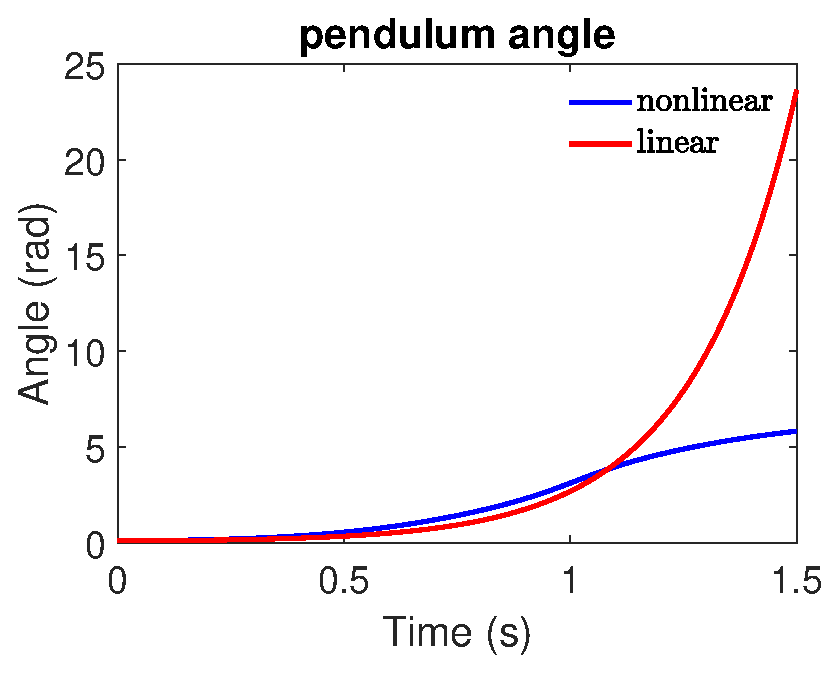
\includegraphics [width=4in]{open_loop_01.eps}

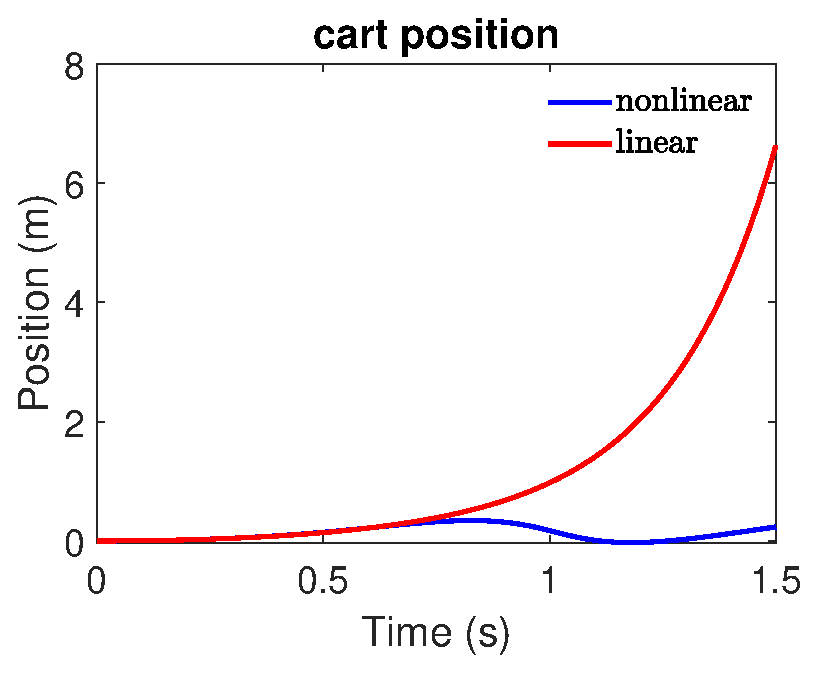
\includegraphics [width=4in]{open_loop_02.eps}



\end{document}

